\section{Лекция 2 -- 2024-02-16 -- }

\subsection{Классификация состояний марковской цепи}

\begin{ex}
  Рассмотрим вот такую марковскую цепь, состоящую из двух состояний:
  \begin{figure}[h!]
    \centering
    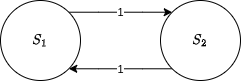
\includegraphics[width=0.2\linewidth]{Figures/lec2-ex1}
  \end{figure}
 
  Для неё:
  \[
    P = \begin{pmatrix}
      0 & 1 \\
      1 & 0
    \end{pmatrix},
    P^{2n + 1} = \begin{pmatrix}
      0 & 1 \\
      1 & 0
    \end{pmatrix},
    P^{2n} = \begin{pmatrix}
      1 & 0 \\
      0 & 1
    \end{pmatrix},
  \]
  очевидно, такая последовательность не может иметь предела, поэтому такая марковская цепь не
  эргодичная.

  Однако, в этой марковской цепи существует стационарное распределение: СЛАУ
  $\pi^T = \pi^T P, \sum \pi_j = 1$ даёт решение $\pi^T = (0.5, 0.5)$.
\end{ex}

\begin{ex}
  Рассмотрим марковскую цепь, состоящую из состояний некоторого устройства. Пусть первое 
  состояние -- работоспособное устройство, второе и третье -- чуть поломанное (можно починить),
  четвертое -- сломано полностью (такое устройство списывают).
  \begin{figure}[h!]
    \centering
    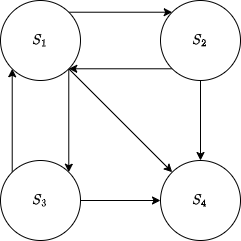
\includegraphics[width=0.3\linewidth]{Figures/lec2-ex2}
  \end{figure}
  
  стрелочками помечены ненулевые вероятности (для примера не важно какие).
  \[
    P = \begin{pmatrix}
      \dots \\
      \dots \\
      \dots \\
      0 & 0 & 0 & 1
    \end{pmatrix} 
  \]
  и тогда $p = (0, 0, 0, 1)$ является стационарным распределением.
  И интуитивно понятно, что начиная с любого состояния рано или поздно сломаемся.
  Данная марковская цепь не является эргодической.
\end{ex}

\begin{ex}
  Рассмотрим марковскую цепь:
  \begin{figure}[h!]
    \centering
    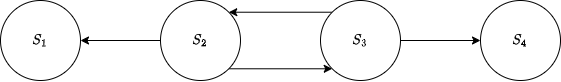
\includegraphics[width=0.5\linewidth]{Figures/lec2-ex3}
  \end{figure}
  
  Для данной марковской цепи стационарными распределениями будут являтся $(1, 0, 0, 0)$
  и $(0, 0, 0, 1)$. Она тоже не является эргодической, так как нет финальных вероятностей.
\end{ex}

\begin{definition}
  Состояние $S_i$ (или множество состояний) называется \emph{несущественным}, если
  $\exists S_j, \exists n : p_{ij}^{(n)} > 0$ -- из этого состояния можно выйти,
  но $\forall S_j, \forall n : p_{ji}^{(n)} = 0$ -- в это состояние нельзя попасть.
\end{definition}

\begin{definition}
  Состояние (или множество состояний) называется \emph{поглощающим}, если в него можно войти --
  $\exists S_j , \exists n : p_{ji}^{(n)} > 0$,
  но нельзя выйти --
  $\forall S_j, \forall n : p_{ij}^{(n)} = 0$.
\end{definition}

\begin{definition}
  Состояние $S_i$ достижимо из состояния $S_j$, если $\exists n : p_{ji}^{(n)} > 0$.
\end{definition}

\begin{definition}
  Если $S_i$ достижимо из $S_j$, $S_j$ достижимо из $S_i$, то $S_i$ и $S_j$ -- \emph{сообщающиеся
  состояния}.
\end{definition}

Отношение сообщаемости является рефлексивным, транзитивным и симметричным, поэтому оно является 
отношением эквивалентности, тогда отношение сообщаемости разбивает марковскую цепь на классы эквивалентности.

\begin{definition}
  Если марковская цепь состоит из одного класса эквивалентности, то она называется
  \emph{неразложимой}.
\end{definition}

\begin{ex}
  % TODO рисунок
  \[
    P = \begin{pmatrix}
      0 & 0 & 1/2 & 1/2 \\
      0 & 0 & 1/2 & 1/2 \\
      1/2 & 1/2 & 0 & 0 \\
      1/2 & 1/2 & 0 & 0
    \end{pmatrix}; \quad
    P^2 = \begin{pmatrix}
      1/2 & 1/2 & 0 & 0 \\
      1/2 & 1/2 & 0 & 0 \\
      0 & 0 & 1/2 & 1/2 \\
      0 & 0 & 1/2 & 1/2
    \end{pmatrix} 
  \]

  то есть начиная в $S_1$ или $S_2$, попадем в $S_3$ $S_4$, потом назад в $S_1$, $S_2$.
  Такая ситуация называется цикличностью.
\end{ex}

\begin{definition}
  Состояние $S_i$ \emph{имеет период $d(i) = d$}, если
  \begin{enumerate}
    \item $p_{ii}^{(n)} > 0 \Rightarrow n = d \cdot l, l \in \mathbb{N}$ ($n$ делится на $d$).
    \item $d$ -- наибольший общий делитель всех таких $n$, для которых выполнено 1.
  \end{enumerate}
\end{definition}

В примере выше $d(1, 2, 3, 4) = 2$.

\begin{definition}
  Если $d(i) = 1$, то состояние называется \emph{апериодическим}.

  Если $p_{ii}^{(n)} = 0 \, \forall n$, то говорят $d(i) = 0$.
\end{definition}



% Следующая теорема есть в Ширяеве
\begin{theorem}
  Если $S = \left\{ S_1, \dots, S_n \right\} $, марковская цепь неразложима и все состояния
  периодические, то $d(i) = d(j) \, \forall i, j$.
\end{theorem}
\begin{proof}
  Выберем $S_i$ -- периодическое с периодом $d(i)$, $S_j$ -- периодическое с периодом $d(j)$.
  Необходимо доказать, что $d(i) = d(j)$.
  \begin{multline*}
    \begin{cases}
    \exists k : p_{ij}^{(k)} > 0, \\
      \exists l : p_{ji}^{(l)} > 0
    \end{cases}
    \Rightarrow \text{по т-ме Колмогорова-Чепмена: } \\
    p_{ii}^{(k+l)} = \sum_{\alpha} p_{i\alpha}^{(k)} \cdot p_{\alpha i}^{(l)} 
    \geqslant p_{ij}^{(k)} \cdot p_{ji}^{(l)} > 0
    \Rightarrow
    k+l \text{ делится на $d(i)$}.
  \end{multline*}
  если $n$ не делится на $d(i)$, то $n+k+l$ не делится на $d(i)$, тогда $p_{ii}^{(n+k+l)} = 0$, 
  тогда $p_{ii}^{(n+k+l)} = \sum_{\alpha} \sum_\beta p_{i\alpha}^{(k)} p_{\alpha \beta}^{(n)} 
  p_{\beta i}^{(l)}$, тогда $p_{jj}^{(n)} = 0$ тогда $n$ не делится на $d(j)$.

  если $p_{jj}^{(n)} > 0 \Rightarrow$ $n$ делится на $d(i)$, а по предположению теоремы $n$ делится 
  на $d(j)$ $\Rightarrow$ $d(i) \leqslant d(j)$.

  Аналогично можно доказать, что $d(j) \leqslant d(i)$. То есть $d(i) = d(j)$.
\end{proof}

\begin{definition}
  Этот общий период называется периодом цепи $d(S)$.
  Если $d(S) = 1$, то цепь называется апериодической -- все состояния непериодические.
\end{definition}

\begin{theorem}
  Марковская цепь с конечным множеством состояний является эргодической тогда и только тогда,
  когда она апериодична и неразложима.
\end{theorem}
(без доказательства)

\begin{theorem}
  Марковская цепь со счетным множеством состояний является эргодической тогда и только тогда,
  когда она неразложима, апериодична, возвратна и положительна.
\end{theorem}
(без доказательства)

\begin{definition}
  Состояние $S_i$ называется возвратным, если $\sum_{n=1}^{\infty} f_{ii}^{(n)} = 1$,
  где 
  \[
    f_{ii}^{(n)} = P(\xi_n = i, \xi_{n-1} \neq i, \dots, \xi_1 = i | \xi_0 = i).
  \]
\end{definition}

\begin{definition}
  Цепь называется возвратной, если все ее состояния возратны.
\end{definition}

\begin{definition}
  Состояние $S_i$ называется положительным, если $\sum_{n=1}^{\infty} n f_{ii}^{(n)} < \infty$
  (матож < $\infty$, то есть можем вернуться за конечное число шагов).
\end{definition}

\begin{definition}
  Цепь называется положительной, если все ее состояния положительны.
\end{definition}


\begin{ex}
  % TODO рисунок бесконечная гусеница
  $p+q=1$.

  \[
    P = \begin{pmatrix}
      0 & 1 & 0 & \dots \\
      q & 0 & p & \dots \\
      0 & q & 0 & p \\
      \dots
    \end{pmatrix} 
  \]

  Найдём стационарные состояния:
  \[
    \pi^T = \pi^T P \Leftrightarrow
    \begin{cases}
      \pi_0 = q \pi_1, \\
      \pi_1 = \pi_0 + q \pi_2, \\
      \dots \\
      \pi_k = p \pi_{k-1} + q \pi_{k+1}
    \end{cases}
  \]
  такое уравнение является рекуррентным. Применим алгоритм его решения:
  Характеристическое уравнение: $q \lambda^2 - \lambda + p = 0$.
  \[
    \lambda_{1, 2} = \dfrac{1\pm \sqrt{1-4pq}}{2q} = \dfrac{1 \pm \sqrt{1 - 4(1-q)q}}{2q}
    = \dfrac{1 \pm |1 - 2q|}{2q}
  \]
  \begin{enumerate}
    \item $q > \dfrac{1}{2}$ -- движение влево более вероятно, чем вправо.
      \[
        \lambda_{1, 2} = 1, \dfrac{1-q}{q}.
      \]
      $\pi_k = c_1 \cdot 1^k + c_2 \cdot \left( \dfrac{p}{q} \right)^k$.
      Причем $0 < \pi_k < 1$ $\Rightarrow$ и $\sum_{k=0}^\infty \pi_k = 1$.
      Получаем, $C_1 = 0, \sum_{k=0}^\infty C_2 \left( \dfrac{p}{q} \right)^k 
      \Rightarrow C_2 = \dots = \dfrac{q-p}{q}$
      % TODO дописать из семинара

      Получили эргодичность.

    \item $q = \dfrac{1}{2}$ тогда $\lambda_{12} = 1$ -- двукратный корень. $\pi_k = C_1 + C_2 k$. 
      Тогда $\pi_k = 0$. Неэргодичная.

    \item $q<\dfrac{1}{2}$. $\lambda_{1, 2} = \dfrac{1 \pm (1-2q)}{2q} = \dfrac{p}{q}, 1$.
      $\pi_k = C_1 + C_2 \left(\dfrac{p}{q}\right)^{k} \Rightarrow \pi_k = 0$.
  \end{enumerate}
\end{ex}

\begin{definition}
  Пусть конечное множество состояний $S = \left\{ S_1, \dots, S_m \right\} $. Берём подмножество 
  состояний (для определенности первые $m_1 < m$ состояний)
  $A = \left\{ S_1, \dots, S_{m_1} \right\} $.
  Обозначим $H^A = \inf \left\{ n\geqslant 0, \xi_n \in A \right\} $ -- момент первого достижения 
  множества $A$.
  Обозначим $h^A = P(H^A < \infty | \xi_0 = i)$.
  $\mu^A_i = M(H^A | \xi_0 = i)$
\end{definition}

\begin{theorem}
  Если $A \subset S$, то $h_i^A$ -- наименьшее неотрицателььное решение системы.
  \[
    h^A_i = \begin{cases}
      1, S_i \in A \\
      \sum_{j=1}^m p_{ij} h_j^A, S_i \notin A
    \end{cases}
  \]

  $\mu^A_i = 0, S_i \in A$
  $\mu^A_i = 1 + \sum_{j=m_1+1}^{m} p_{ij} \mu_j^A, S_i \notin A$.
\end{theorem}

